% one-figure manuscript written by fig_qc.py --tek-sekil-tex (trap T29)
\begin{figure}[!t]
\centering
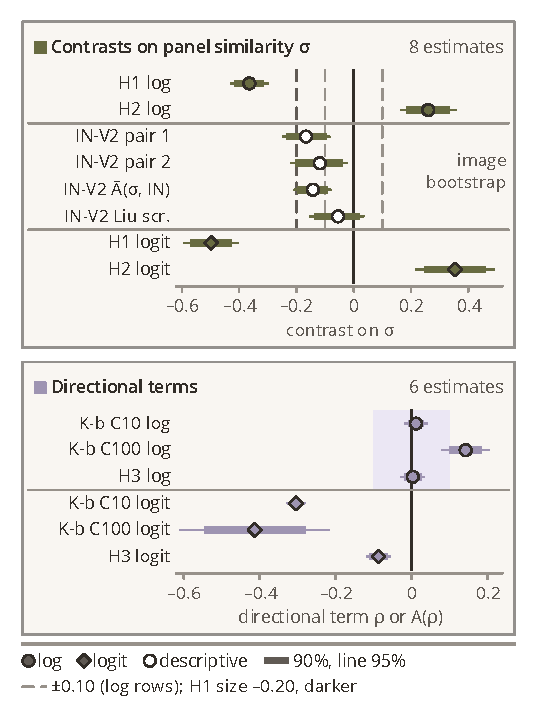
\includegraphics{fig12_estimates_forest}
\caption{\textbf{Registered estimates as two hanging tags.} The upper card, Contrasts on panel similarity σ, holds H1, H2 and descriptive ImageNetV2 rows; the lower card, Directional terms, holds K-b and H3. Circles log, diamonds logit, open marks descriptive; thick and thin bars are 90% and 95% intervals, over images only on ImageNetV2. The ±0.10 lines apply to log rows only.}
\label{fig:fig12_estimates_forest}
\end{figure}
